\newcommand{\dir}{../preface}

%========================= PREFACE ========================= 
\ifthenelse{\boolean{edthesis}}
 {
   \begin{prefacepart}
   \pagenumbering{roman} 
}
{
  \frontmatter
}

\thispagestyle{empty}
\begin{minipage}{\textwidth}
\end{minipage}
\begin{center}
\vspace{2cm}
{ \Huge Statistical Approaches to Viral Phylodynamics
  \par
  \vspace{0.5cm} 
{\Large Luiz Max Fagundes de Carvalho \par}
}
\end{center}
\vfill
\begin{center}
\vspace{6cm}    
\centerline{\epsfig{file=\dir/2Line2ColCMYK_CS3.eps,width=0.35\textwidth}}
\vspace{0.5cm}
Thesis submitted in fulfilment of\\
the requirements for the degree of\\ 
Doctor of Philosophy\\ 
to the\\
University of Edinburgh --- 2018
\end{center}

\newpage
\thispagestyle{empty}
% \nobibliography*
% \bibliographystyle{plainnt}
% \nocite{*}



\chapter{Declaration}
\vspace*{2\baselineskip}
I declare that this thesis has been composed 
solely by myself and that it has not been submitted, either in whole or
in part, in any previous application for a degree.
Except where otherwise acknowledged, the work presented is entirely my
own.
\vspace{6\baselineskip}\\
\begin{flushright}
\hspace*{\fill}
Luiz Max Fagundes de Carvalho
\newline
January 2018
\end{flushright}
\cleardoublepage

\chapter{Abstract}
\markboth{\MakeUppercase{Abstract}}{\MakeUppercase{Abstract}}
The recent years have witnessed a rapid increase in the quantity and quality of genomic data collected from human and animal pathogens, viruses in particular.
When coupled with mathematical and statistical models, these data allow us to combine evolutionary theory and epidemiology to understand pathogen dynamics.
While these developments led to important epidemiological questions being tackled, it also exposed the need for improved analytical methods.
In this thesis I employ modern statistical techniques to address two pressing issues in phylodynamics: (i) computational tools for Bayesian phylogenetics and (ii) data integration.
I detail the development and testing of new transition kernels for Markov Chain Monte Carlo (MCMC) for time-calibrated phylogenetics in Chapter 2 and show that an adaptive kernel leads to improved MCMC performance in terms of mixing for a range of data sets, in particular for a challenging Ebola virus phylogeny with 1610 taxa/sequences.
As a trade-off, I also found that the new adaptive kernels have longer warm up times in general, suggesting room for improvement.
Chapter 3 shows how to apply state-of-the-art techniques to visualise and analyse phylogenetic space and MCMC for time-calibrated phylogenies, which are crucial to the viral phylodynamics analysis pipeline.
I describe a pipeline for a typical phylodynamic analysis which includes convergence diagnostics for continuous parameters and in phylogenetic space, extending existing methods to deal with large time-calibrated phylogenies.
In addition I investigate different representations of phylogenetic space through multi-dimensional scaling (MDS) or univariate distributions of distances to a focal tree and show that even for the simplest toy examples phylogenetic space remains complex and in particular not all metrics lead to desirable or useful representations.
On the data integration front, Chapters 4 and 5 detail the use data from the 2013-2016 Ebola virus disease (EVD) epidemic in West Africa to show how one can combine phylogenetic and epidemiological data to tackle epidemiological questions.
I explore the determinants of the Ebola epidemic in Chapter 4 through a generalised linear model framework coupled with Bayesian stochastic search variable selection (BSSVS) to assess the relative importance climatic and socio-economic variables on EVD number of cases.
In Chapter 5 I tackle the question of whether a particular glycoprotein mutation could lead to increased  human mortality from EVD.
I show that a principled analysis of the available data that accounts for several sources of uncertainty as well as shared ancestry between samples does not allow us to ascertain the presence of such effect of a viral mutation on mortality.
Chapter 6 attempts to bring the findings of the thesis together and discuss how the field of phylodynamics, in special its methodological aspect, might move forward.
% \setlength{\voffset}{-1.75in}
\chapter{Acknowledgements}
\markboth{\MakeUppercase{Acknowledgements}}{\MakeUppercase{Acknowledgements}}

Many people have, in one way or another, contributed for me to be in a position to do the research I describe in this thesis.
From the servitor to the cleaning staff to numerous fellow scientists that during millennia pursued Truth, and on whose mighty shoulders I have stood.
Andrew Rambaut is one of these rare people that possess both a powerful intellect and a kind soul.
For his generosity in dedicating countless hours to discussing various aspects of my research and helping me grow as scientist, I'm thankful.
Special thanks are in order to Gytis Dudas, Darren Obbard, Jarrod Hadfield, Richard Whittet, Tom Booker, Trevor Bedford, Matthew Hall, Guy Baele, Philippe Lemey and Marc Suchard for stimulating discussions.
Thanks to Lisa for single-handedly handing in this thesis.

I could acknowledge a bunch of my plonker friends by name, but this would inevitably lead to me forgetting someone(s) and getting in trouble.
So I won't.
You know who you are.
My loving wife's support was vital over these arduous years.
To you, \textit{Tatu}, I'm very very grateful.
The unwavering support of my parents and siblings not only during my PhD but throughout my whole life helped me realise my boyhood dream: becoming a professional scientist.

The quotes at the beginning of each chapter are loosely related with the topic of the chapter in question, but don't waste your time trying to make a connection if one is not obvious to you; chances are it only makes sense to myself.


{\setlength{\parskip}{0ex plus 0.5ex minus 0.2ex}

\ifthenelse{\boolean{edthesis}}
 {
  \begin{singlespace}
 }{}

\tableofcontents
\listoftables
\listoffigures
% Glossary stuff
%\input{\dir/glossary.tex}
%\cleardoublepage
%\renewcommand{\nomname}{List of Symbols}
%\markboth{\MakeUppercase{\nomname}}{\MakeUppercase{\nomname}}
%\addcontentsline{toc}{chapter}{List of Symbols}
%\printglossary
\ifthenelse{\boolean{edthesis}}
 {
  \end{singlespace}
 }{}
}

\ifthenelse{\boolean{edthesis}}
 {
   \end{prefacepart}
   \pagenumbering{arabic} 
}
{
   \mainmatter
}
%========================= CHAPTERS ========================= 
\renewcommand{\dir}{../chapter1/chapter/}
\chapter{Template Chapter}
This is a template chapter. Lots of exciting stuff should go in here\footnote{testing a footnote}.


\begin{figure}[htbp]
  \centering
  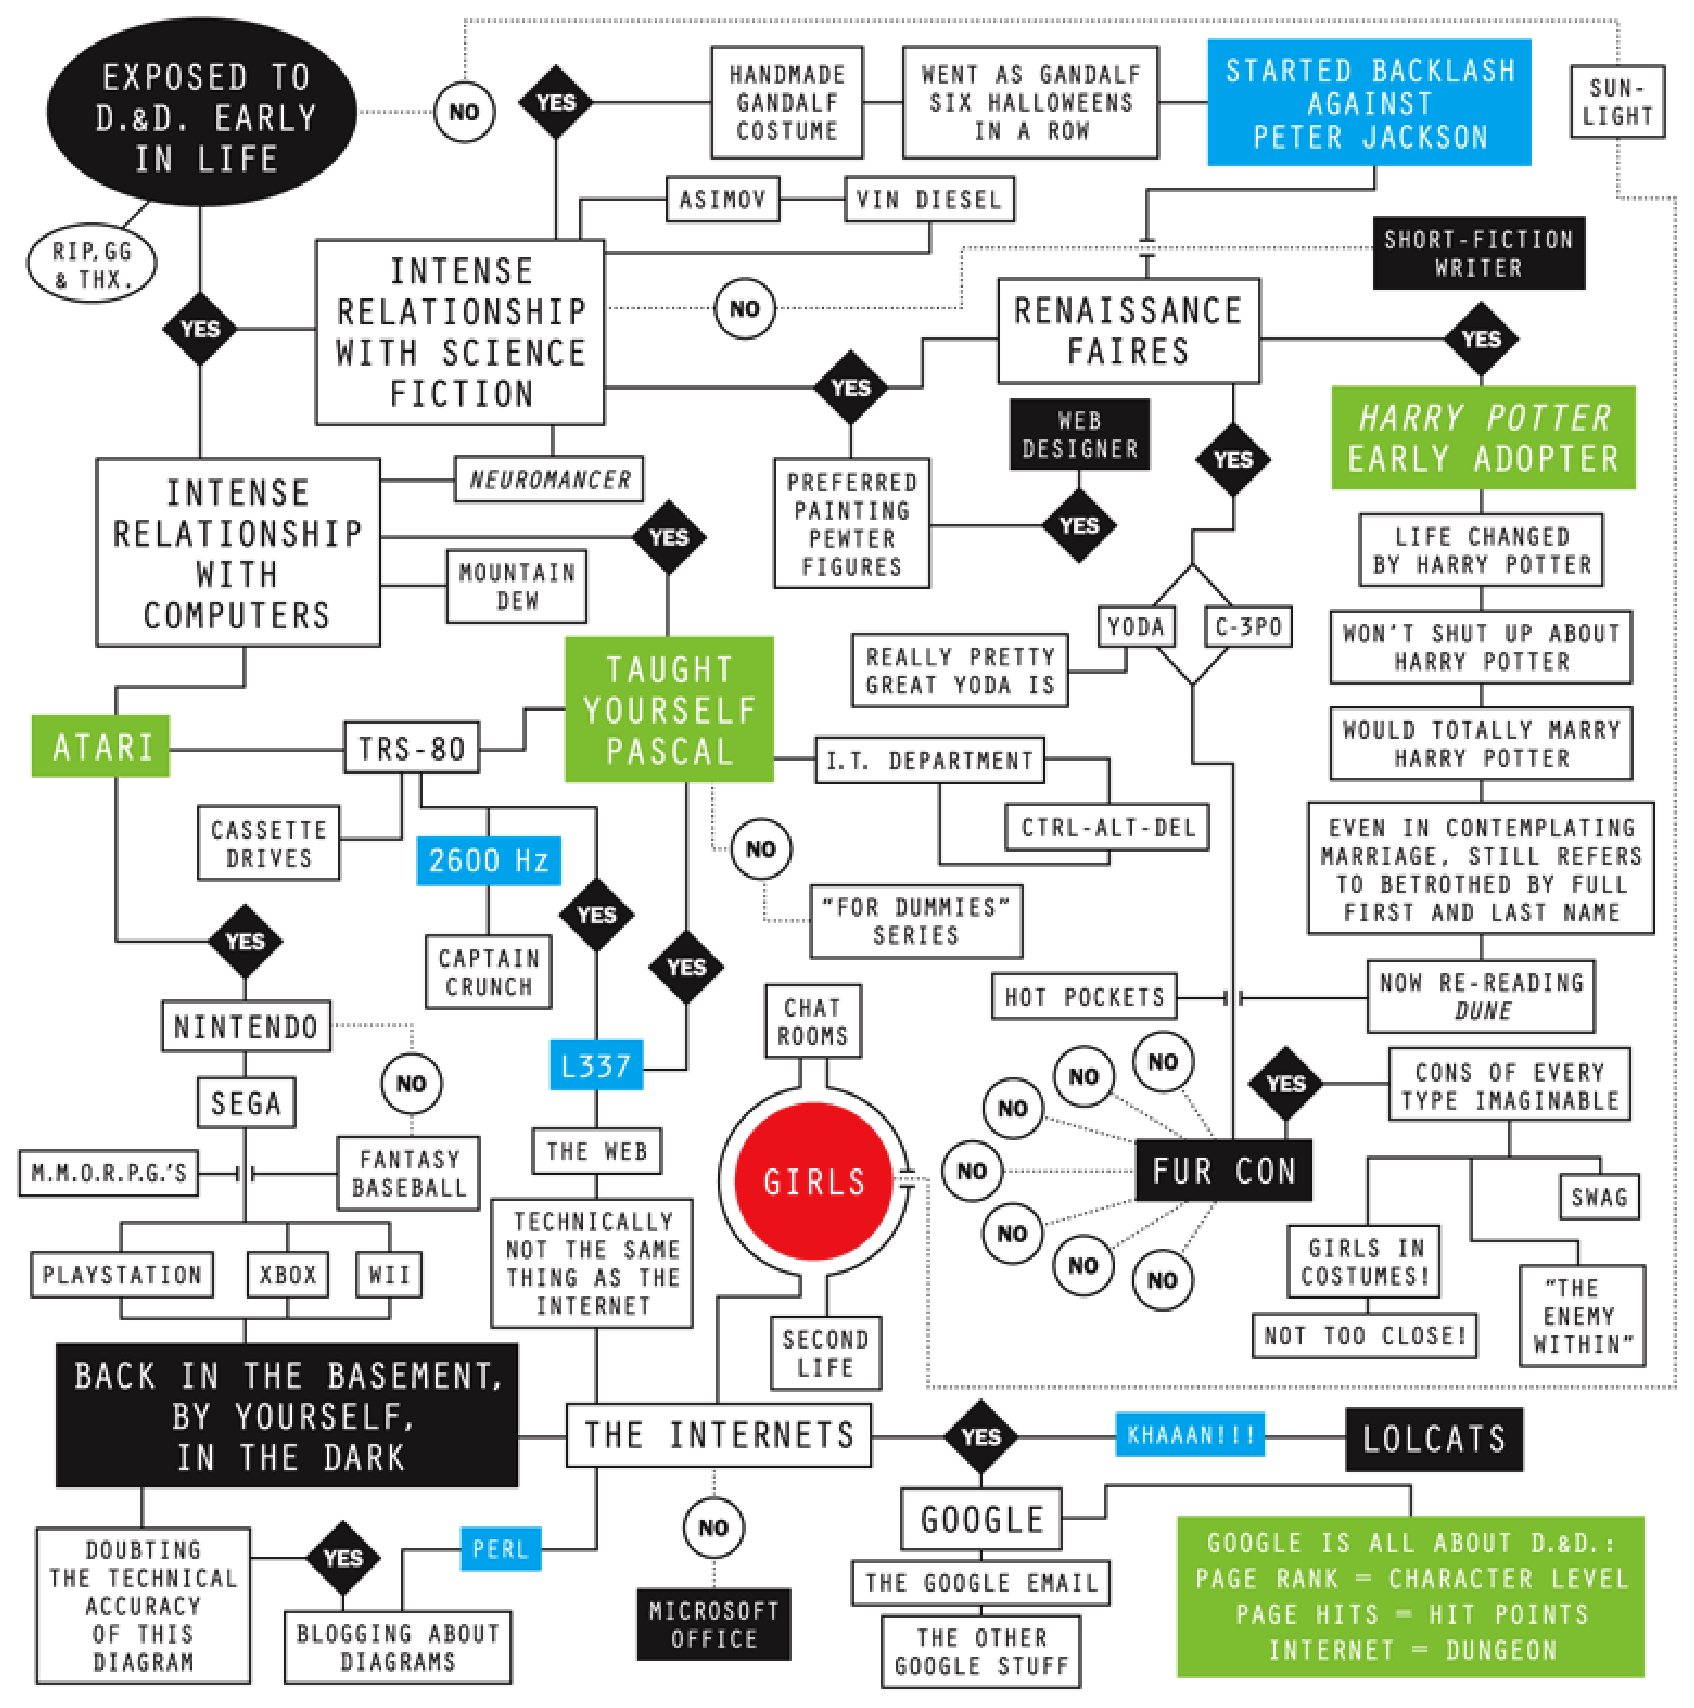
\includegraphics[width=0.7\textwidth]{\dir/figs/geek_flow_chart_nyt.eps}
  \caption{an example figure...}
  \label{fig.example}
\end{figure}

\renewcommand{\dir}{../chapter2/chapter/}
\chapter{Adaptive time-tree transition kernels for Bayesian phylogenetics}

\section{Introduction}	
\label{sec:intro}

The use of Markov chain Monte Carlo (MCMC) for Bayesian methods in phylogenetics has grown steadily since its introduction in the late 1990s and early 2000s~\citep{Rannala1996, Yang1997, Mau1999, Li2000}, with software packages such as Mr Bayes~\citep{Ronquist2012} and BEAST~\citep{Drummond2012} becoming widely used by researchers in a broad range of disciplines~\citep{Murphy2001, Bouckaert2012, Lemey2014}.
% \citep{sinsheimer1996bayesian} is probably the first use of Bayesian methods in phylogenetics.

In Bayesian phylogenetics one is usually interested in computing the posterior distribution
\begin{equation}
\label{eq:posterior}
 p(t, \boldsymbol b, \boldsymbol \theta | D) = \frac{f(D | t, \boldsymbol b, \boldsymbol \theta ) \pi(t, \boldsymbol b, \boldsymbol \theta )}{\sum_{t_i \in \boldsymbol T} \int_{\boldsymbol B}\int_{\boldsymbol \Theta} f(D | t_i, \boldsymbol b_i, \boldsymbol \theta ) \pi(t_i, \boldsymbol b_i, \boldsymbol \theta ) d\boldsymbol\theta d\boldsymbol b_i}\:,
\end{equation}
where $D$ is observed data, $\boldsymbol T$ is the set of all binary rooted trees and $t \in \boldsymbol T$  is a tree topology associated set of branch lengths $\boldsymbol b$.
Finally $\boldsymbol \theta$ is a set of parameters of interest such as substitution model parameters, migration rates, heritability coefficients, etc.

In many applications, interest lies in constructing time-calibrated phylogenies, i.e. phylogenetic trees whose branch lengths are measured in units of calendar time.
In particular, one might have sequences sampled through time (heterochronous) which enable direct estimation of the rate of evolution and reconstruction of past population dynamics~\citep{Drummond2002, Drummond2005}.
These types of data sets pose additional challenges to inference because they impose constraints on the space of valid trees~\citep{Stadler2013}.

One of the main features of the Bayesian  approach is to  allow parameter inference and hypothesis testing whilst accommodating phylogenetic uncertainty~\citep{Suchard2001, Huelsenbeck2002}.
This treatment of uncertainty is achieved by integrating over the space of phylogenies, which depends crucially on efficiently traversing tree space.
Even for the simplest models, the distribution in~(\ref{eq:posterior}) cannot be computed analytically, requiring numerical approximation, usually  accomplished through MCMC.

The Metropolis-Hastings (M-H) algorithm~\citep{Metropolis1953, Hastings1970} is a very popular MCMC technique due to its generality and ease of implementation.
In M-H, a Markov chain is constructed such that its limiting distribution is the desired posterior distribution. 
For ease of presentation, let $\tau = \{ t, \boldsymbol b\}$ and $q_{\gamma}(\tau^\prime|\tau)$ be a conditional distribution indexed by a parameter $\gamma$ from which a new state $\tau^\prime$ can be proposed from a current state $\tau$, which we call a \textbf{tree transition kernel}. 
It can be shown that accepting/rejecting a new state $\tau^\prime$ based on the ratio $A_{\gamma}(\tau | \tau^\prime) = min\left(1, \frac{p(\tau^\prime | D)q_{\gamma}(\tau|\tau^\prime)}{p(\tau | D)q_{\gamma}(\tau^\prime|\tau)}\right)$ leads to the desired distribution for a suitably constructed tree transition kernel.

An important thing to notice is that there are no ``default'' choices for the proposal distribution $q_{\gamma}(\cdot|\cdot)$; it must be chosen with the target posterior in mind.
Moreover, the efficiency of MCMC algorithms in approximating the target distribution depends crucially on the choice of transition kernel~\citep{Brooks2003,AlAwadhi2004,Yang2013}.
As argued by~\cite{Hoehna2012}, tree transition kernels are usually built in a relatively simplistic fashion, which in turn leads to inefficient exploration of tree space.
Moreover, most transition kernels proposed to date are not adaptive, i.e., the parameter(s) $\gamma$ cannot be adjusted during the Markov chain to achieve a desired acceptance probability.
Given the clear advantage of adaptive MCMC over non-adaptive implementations for high-dimensional target distributions~\citep{Roberts2009, Baele2017}, the development of adaptive tree transition kernels could lead to substantial gains in performance.

\cite{Lakner2008} were the first to systematically investigate transition kernel efficiency in MCMC for Bayesian phylogenetics.
They investigated the performance of seven kernels on a collection of 10 real-world data sets.
To quantify performance, the authors looked at the percentage of converged runs per tested kernel, using clade frequencies relative to a reference (golden) run as a criterion.
In addition, time to convergence was also used as performance criterion.

\cite{Hoehna2008} developed new ``clock-constrained'' transition kernels to improve efficiency when dealing with time-calibrated trees. 
The authors argue that clock-constrained trees impose additional restrictions on the state space of the MCMC algorithm and hence that performance could be increased by developing transition kernels that took the extra information provided by tip dates.
They develop two such kernels: Fixed node-height Prune-and-Regraft (FNPR) and Intermediate Exchange (IE).
FNPR finds a ``target'' node (excluding the root and its two daughters) at random, prunes it and regrafts the resulting subtree at a ``destination'' node in the tree at the same height at random.
Intermediate Exchange is similar in spirit, but the regraft node  is not chosen at random. 
Instead, IE is constructed to prefer local rearrangements, by picking closer nodes with a higher probability (see below and section II in~\cite{Hoehna2008} for details).
A limitation of FNPR nor IE is that they are not adaptive.

\cite{Hoehna2012} explored more sophisticated ``guided'' tree transition kernels, inspired by Gibbs sampling.
The idea behind their ``metropolised'' Gibbs samplers is to maximise transition probability, i.e., the probability that the chain moves to a new state.
This is accomplished by prohibiting the current state as a proposed state, leading to a transition probability of one.
The kernels developed in~\cite{Hoehna2012} use a weighting scheme based on conditional clade probabilities (CCP) to guide transitions between trees.
A move to a tree with a lower CCP score is thus less likely, whilst a move that increases the score has a higher probability of being accepted.
A limitation of these metropolised transition kernels is that CCP scores require normalisation over all trees~\citep{Larget2013} and hence can be cumbersome to calculate.

To achieve maximum efficiency, a tree transition kernel needs to have the following characteristics: (i) be computationally cheap; (ii) be adaptive; (iii) traverse tree space quickly.

In this paper we develop and study a suite of simple, adaptive time-tree transition kernels, which we implement in the open source software package BEAST (\url{https://github.com/beast-dev/beast-mcmc/}).
We analyse performance in real as well as simulated data sets, focusing on the inference of time-calibrated phylogenies.


\section*{New time-tree transition kernels}


\section*{Results}

\begin{figure}[htbp]
  \centering
  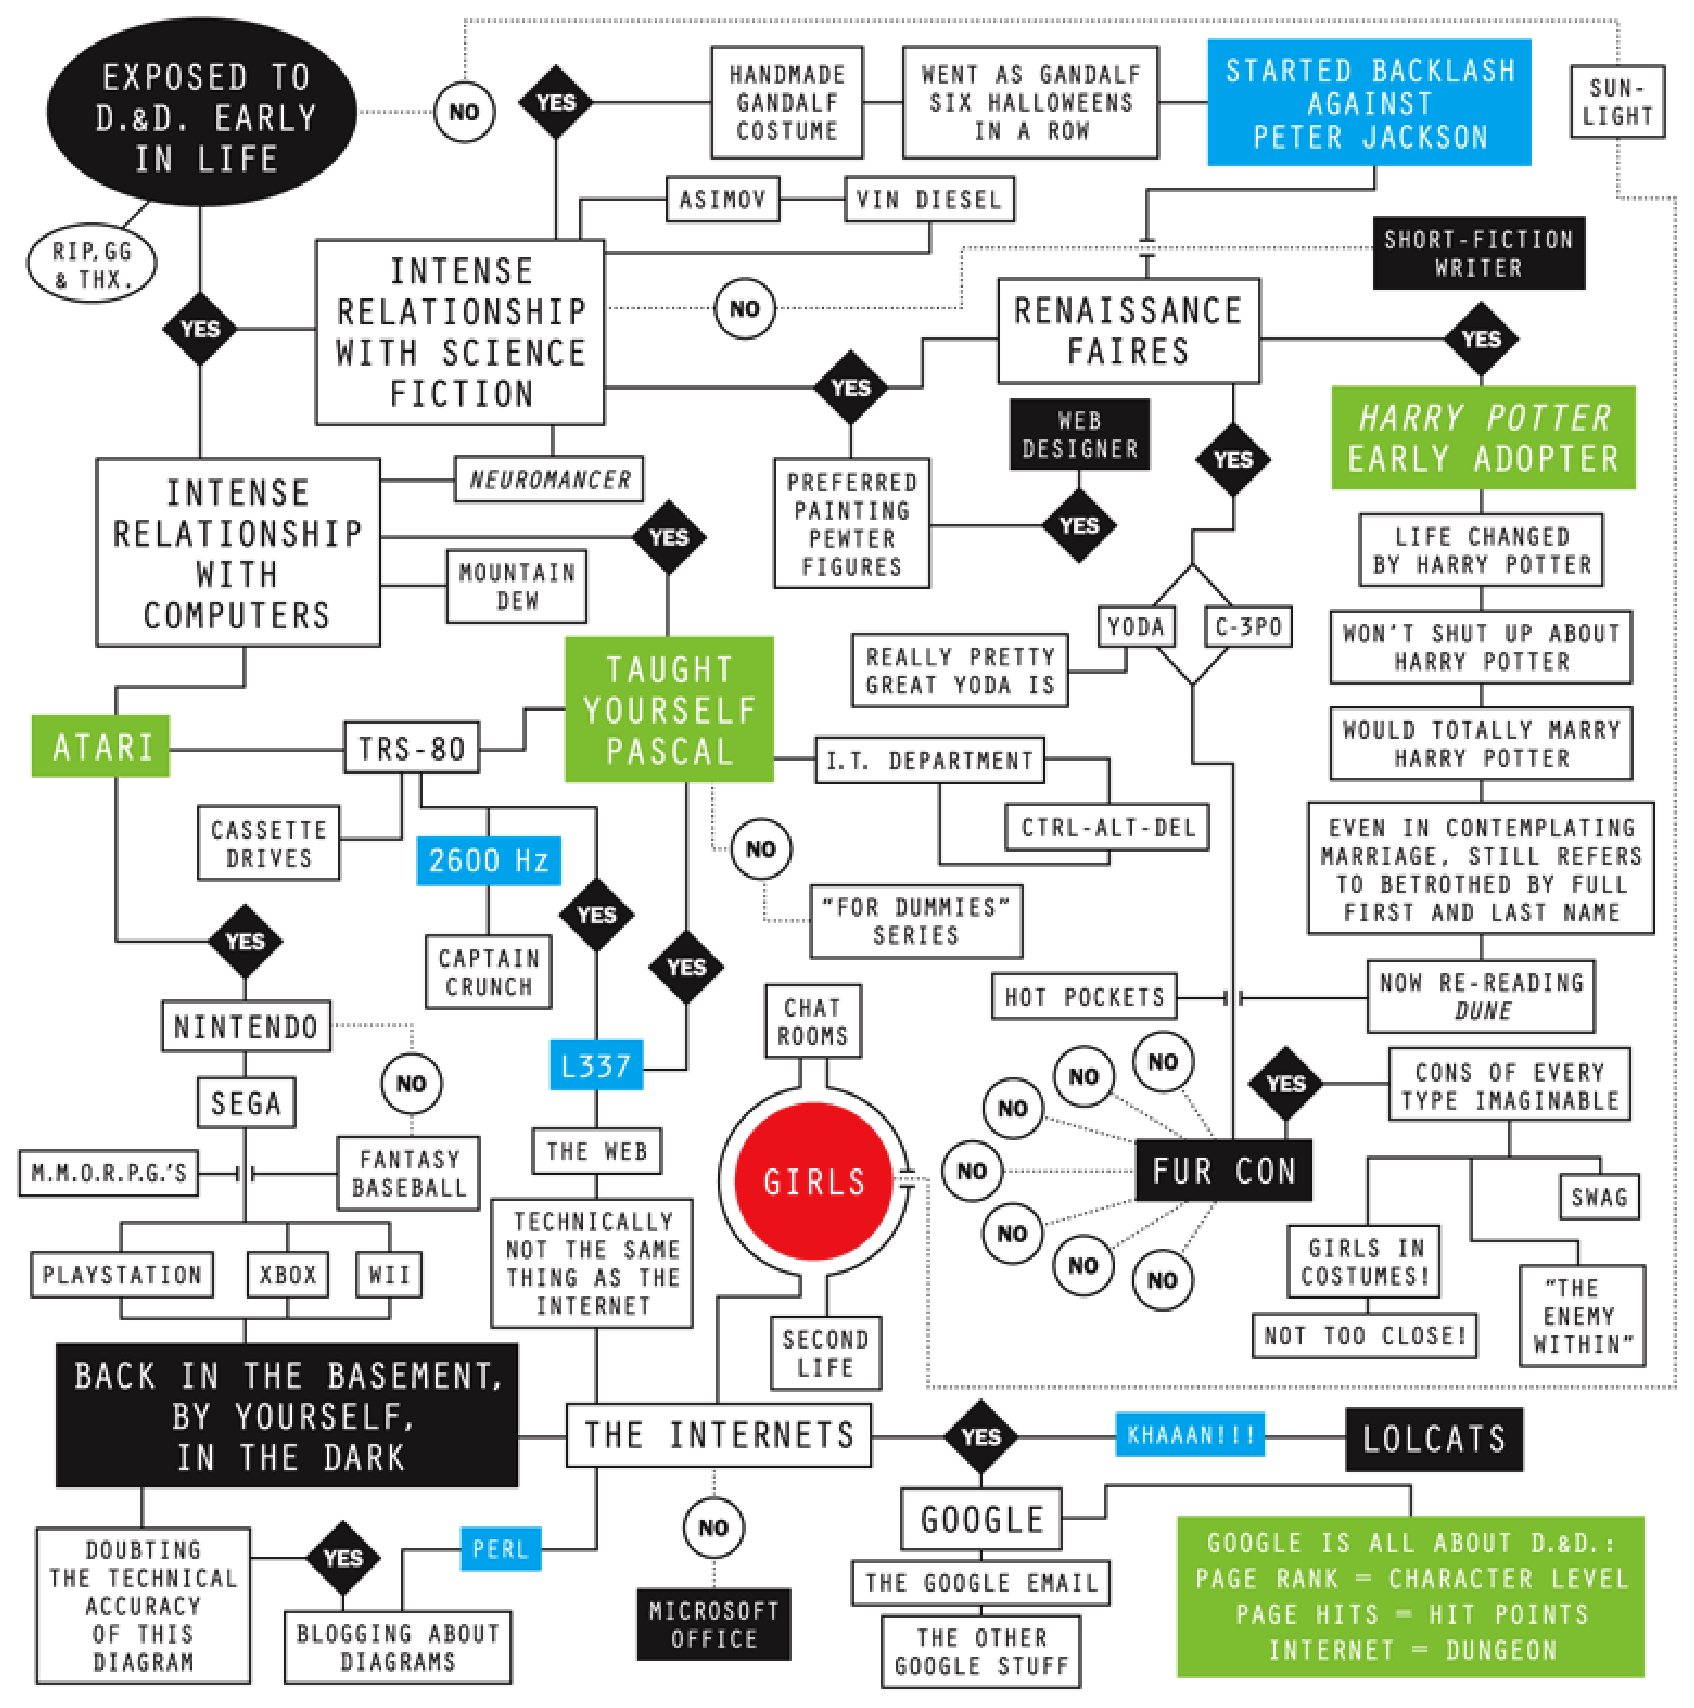
\includegraphics[width=0.7\textwidth]{\dir/figs/geek_flow_chart_nyt.eps}
  \caption{an example figure...}
  \label{fig.example}
\end{figure}

% \bibliography{/home/max/Dropbox/PHD/THESIS/bibliography/lmcarvalho_PhD_Thesis}


%========================= Appendix ========================= 
\renewcommand{\chaptermark}[1]{%
 \markboth{\MakeUppercase{%
 \appendixname} \ \thechapter.%
 \ #1}{}}
%\renewcommand{\dir}{../appendix/appendix}
%\input{\dir/appendix.tex}

%========================= BIBLIOGRAPHY ========================= 
\ifthenelse{\boolean{edthesis}}
 {
 \begin{singlespace}
}
{
  \backmatter
}
%\def\bibname{References}
%\tocotherhead{References}
%\addcontentsline{toc}{chapter}{References}
%\bibliography{ism}
\ifthenelse{\boolean{edthesis}}
 {
  \end{singlespace}
 }{}

